\documentclass[oneside]{article}
\usepackage{fullpage}
\usepackage[pdftex]{graphicx}
\DeclareGraphicsExtensions{.png,.pdf}
\graphicspath{{images/}}
\usepackage{hyperref}
\usepackage{verbatim}
\usepackage[format=plain,font=small]{caption}
\usepackage[small]{titlesec}
\usepackage[round,sectionbib]{natbib}
\usepackage{amstext}
\bibliographystyle{plainnat}
\renewcommand\rmdefault{bch}
\linespread{1.07} 

\newcommand\amin{\text{minor}}
\newcommand\amaj{\text{major}}

\begin{document}

\title{Glyph-maps for visualizing climate data and models}
\author{Cook, Hofmann, Wickham, Wickham}

% Drawing trend lines on map
%   - How to
%   - Comparison to coloring slope
%   - Reference to Grinstein icon plots
% Pickett RM and Grinstein GG (1988). Iconographics 
% displays for visualizing multidimensional data. 
% In Proc. IEEE Conference on Systems, Man, and Cybernetics, pages 514-19.
% Note the later work on metaphoric data display, garbage work!
%   - Alexander Gribov's work http://rosuda.org/software/Gauguin/gauguin.html

%   - Spatial star plots by Andrews http://www.udallas.edu:8080/~andrews/software/software.html
%   - Look at what Bertin does
%
% Interactive graphics
% Data processing
%
% Perhaps the GHCN data? Not gridded
% NOAA data, almost grid, but over ocean, so maps more tricky
% NARCAP from NCAR?
% Fill in with NASA data, to start, try to put new data for final version
\maketitle

\section{Introduction}

Climate data is composed of measurements on variables such as temperature, precipitation, and winds that have been collected from a spatial and temporal context. The classic display for spatial data is to use color or grey scale overlaid on geographic location, typically including a map. When measurements are made at different time periods it is common to display the data as small multiples, such as in Figure \ref{fig:facetted-map}. In this plot, a separate map is drawn for each month (columns) and year (rows), over a 6 year period of remotely sensed temperature data above Central America. Color is used to display the de-seasonalized temperature measurements, with red being high values and blue being low values. The data comes from \citet{murrell:2010}. The most noticeable feature in this display is the strong red in the equatorial region beginning in mid-1997 and tapering out during 1998. This is the pattern of an El Ni\~no event, a major temperature anomaly. With some work other smaller more localized patterns can be perceived, for example, cooler over the land mass in the early year, but warmer in the latter years. What the reader is required to do is play the game ``Spot the difference'' from one small image to another. From a cognitive perspective, this is a very hard task to do. It falls into the framework of {\it change blindness} (see e.g. \citet{healey:2011} and often leads to failure without readers realizing, in particular for small areas of change or subtle changes.  Large structures such as the El Ni\~no event are clear but readers will not be able to effectively glue the images together sufficiently to read off the trend over the years or notice small local deviations between plots. Rendering these small multiples as movie helps with picking up strong trends, but small trends still fail to draw readers' attention and escape unnoticed \citep{simons:gradual}.

\begin{figure*}[htp]
\centerline{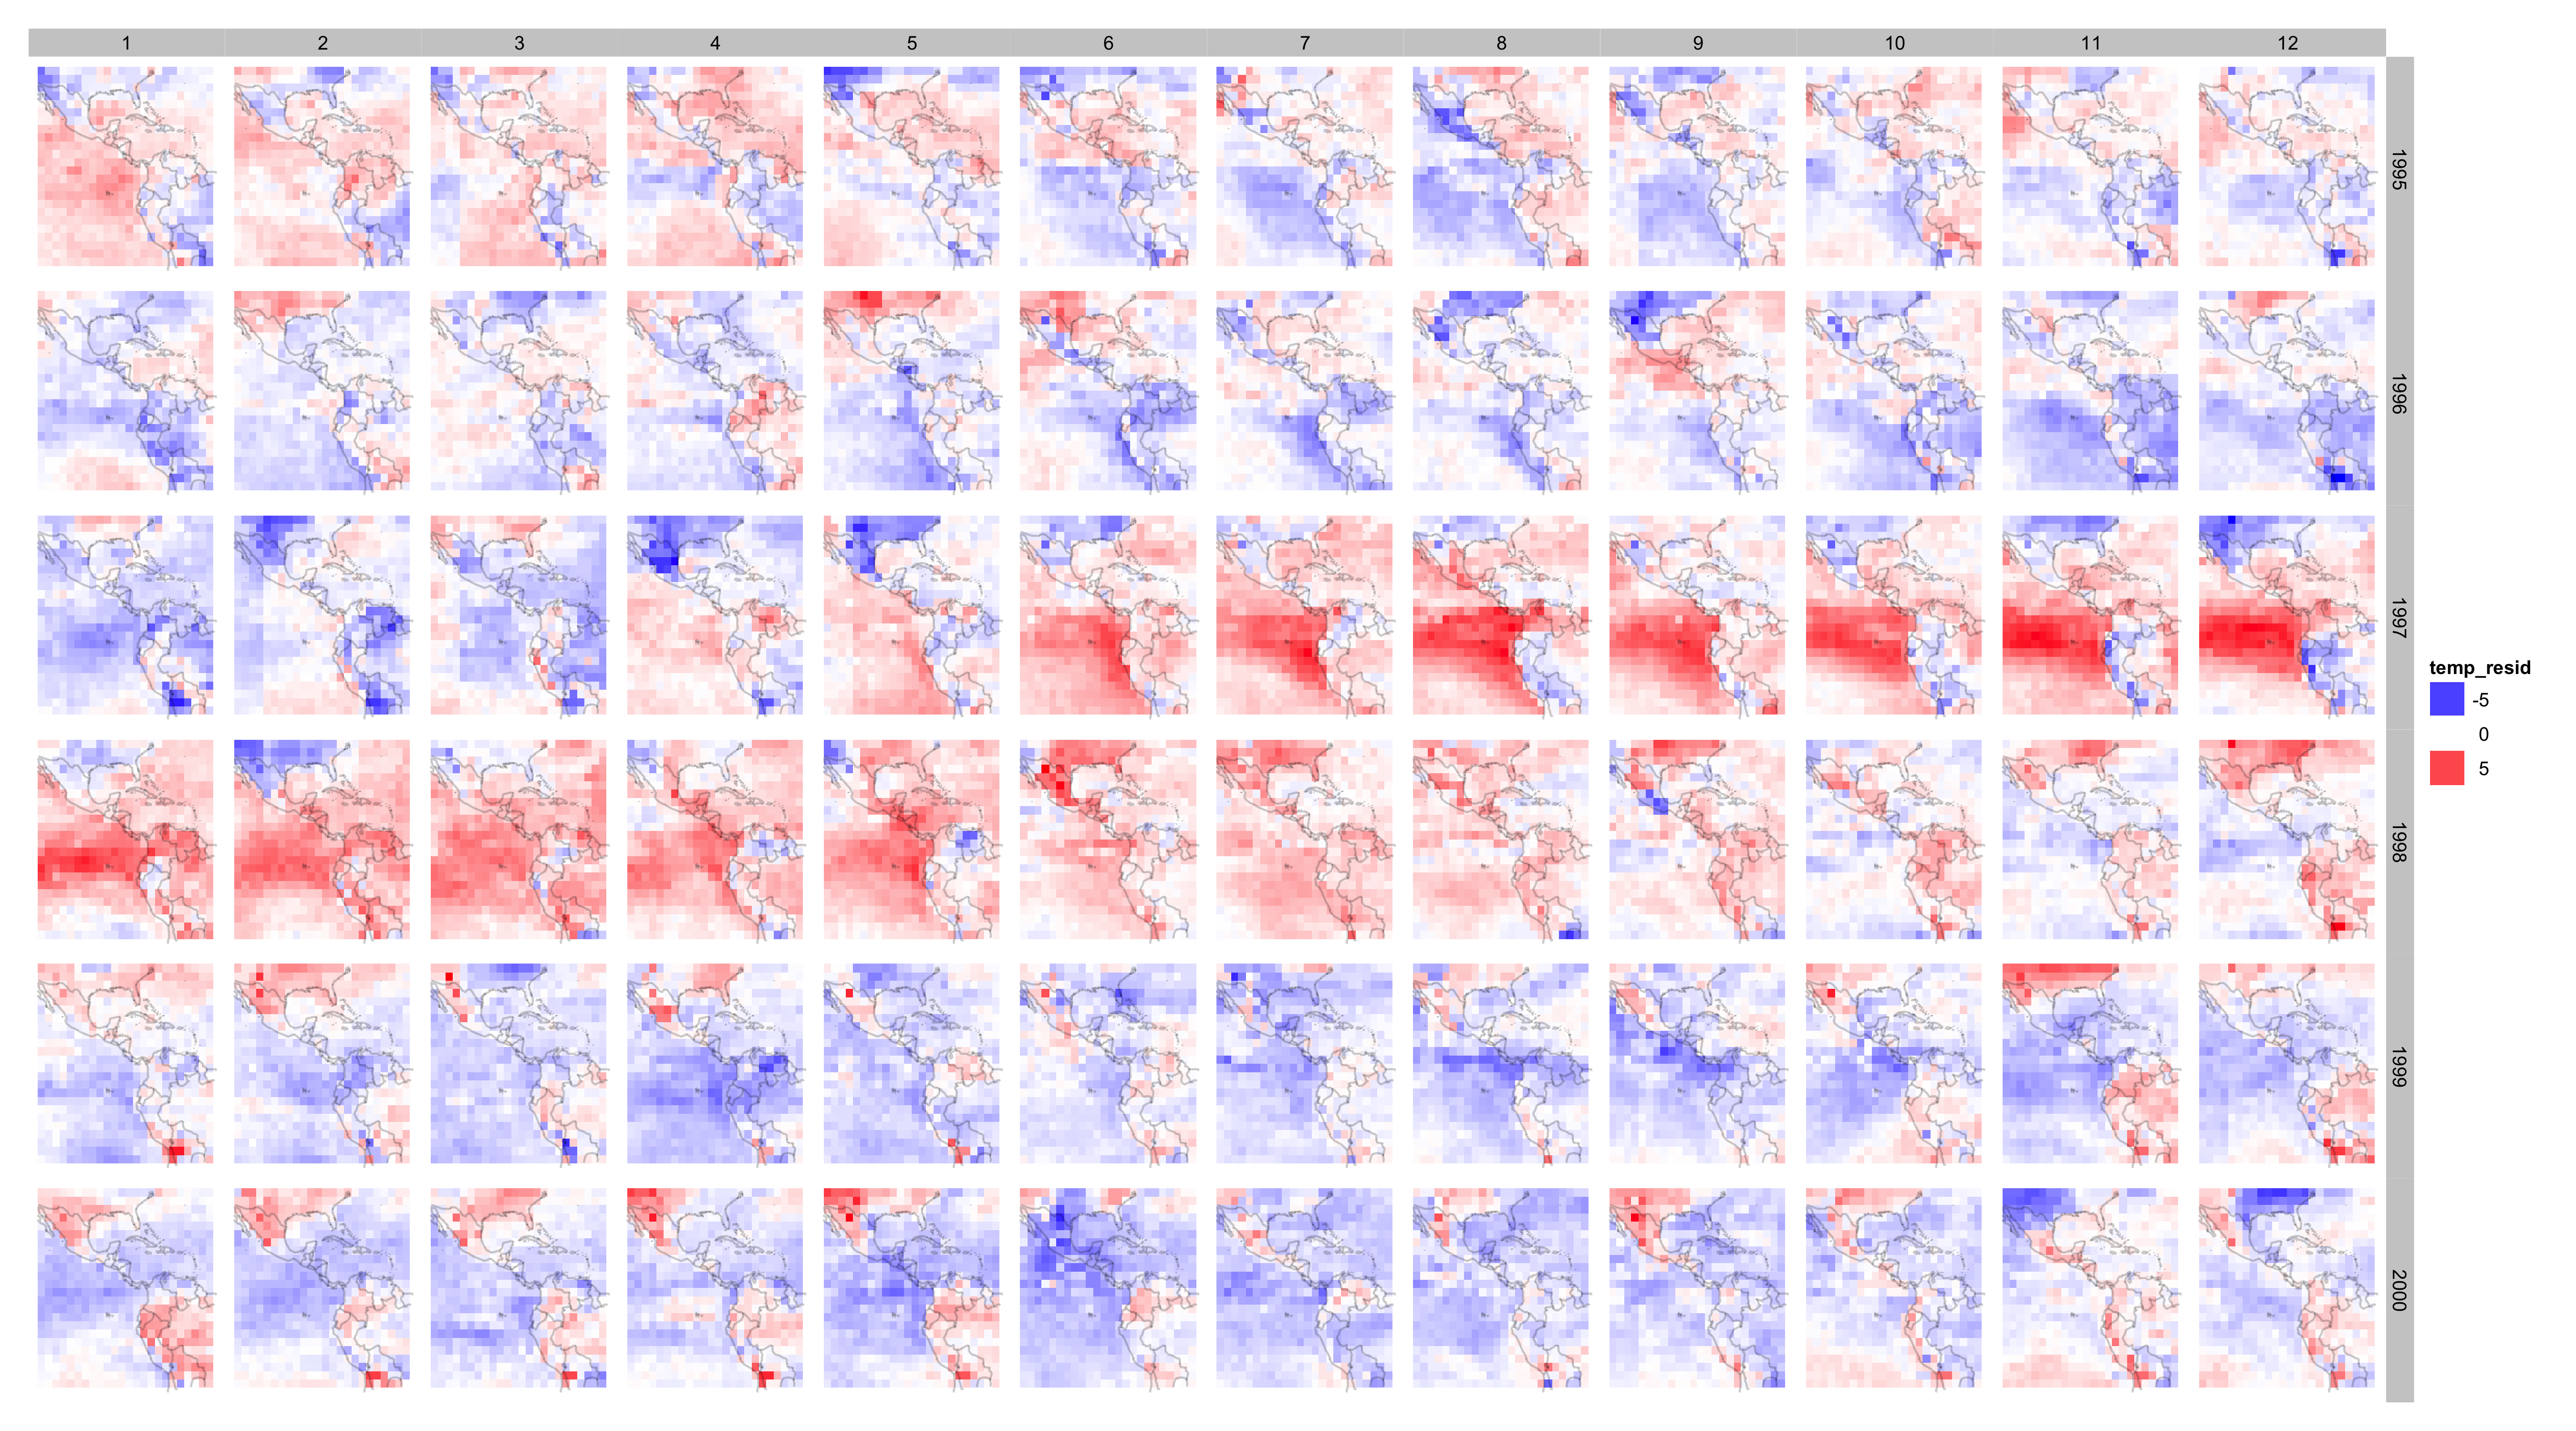
\includegraphics[width=6in]{nasa-colored-map.png}}
\caption{Facetted map of de-seasonalized temperature.}
\label{fig:facetted-map}
\end{figure*}

%% Reproduce all of the icon displays using the fixed glyph code

In this paper we explore the use of a different type of display, that uses icons on the map, for climate data.  Icon plot associated with weather maps date back as far as \citet{galton:weathermap}, described in \citet{friendlydenis:2001}. Icon plots date back to the star plot introduced by \citet{mayr:1877}, and resurged in the modern era with the semi-graphic displays of \citet{anderson:1960}, and were made infamous by \citep{chernoff:1973}. An icon is produced by mapping each variable to some feature of the icon. One icon is generated for every case in the data set. Figure \ref{fig:glyphs} illustrates the construction of star plot, with emphasis on temporal data. The time measurements are treated as variables in a multivariate data set. Variables are Here we have six years of monthly data, giving 72 time values which are considered to be 72 variables. The star plot is formed by considering the 72 axes radiating from a common midpoint, and the data values for the row are plotted on each axis relative to the locations of the minimum and maximum of the variable. For the temporal data, all variables are considered to be on a common scale so the global minimum and maximum of temperature are used to scale each data value. Three different locations are selected, for demonstration purposes. The top plot shows the time series of these three locations. Location ``1.1'' (red) has medium values of temperature, with strong seasonality, the six years corresponding to the six peaks. Location ``2.1'' (green) has generally high temperature values, with weaker seasonality in most years and a lack of low temperatures in the middle of the time period when lows would be expected. Location ``3.1'' (blue) has strong seasonality but generally low temperatures. The bottom plot shows these same cases as star glyphs. A separate glyph is created for each location. The 72 time variables form axes organized radially. Each temperature value is plotted relative to the overall range of temperature values. The seasonal patterns are clearly visible in this type of display, forming six ``petals'' in the icon. Location ``2.1'' has a different pattern than the other two, with only four petals, and location ``3.1'' is a much smaller icon indicating overall lower values. 

\begin{figure*}[htp]
\centerline{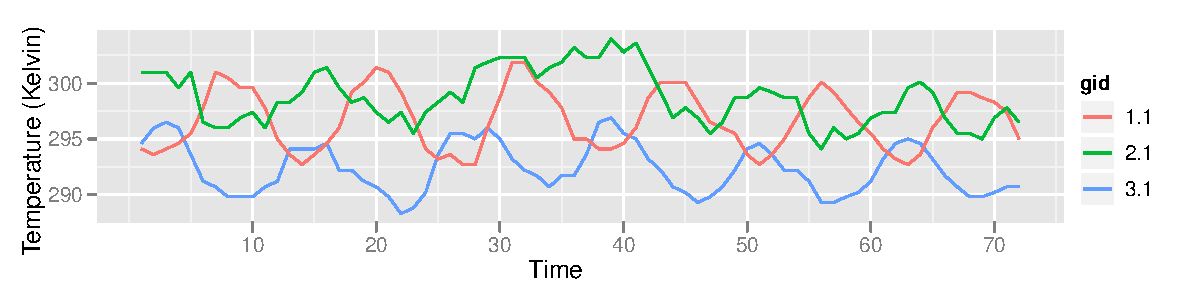
\includegraphics[width=6in]{nasa-glyph-ts.pdf}}
\centerline{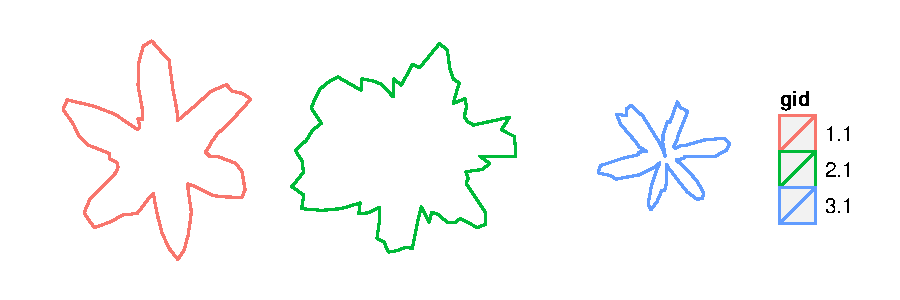
\includegraphics[width=6in]{nasa-glyph.pdf}}
\caption{Icons of raw temperature for three different locations.}
\label{fig:glyphs}
\end{figure*}

Icon plots are used, infrequently, to examine multivariate data. For large data sets it is infeasible to digest the quantity of icons, and for multivariate data there is no natural order so it can be like having a mountain of little stamps to rearrange and organize, in order to understand the structures present in the data. An early paper on multivariate graphics \citep{kleiner:1981} and a recent paper \citep{hurley:2010} propose some approaches for organizing the icons. Ordering of icons is not an issue with spatiotemporal data, because it is naturally handled by spatial location. The spatial trend, or continuity, usually gices the plot an appearance of texturing on a landscape, make it easier to digest patterns among the icons.

Figure \ref{fig:glyph-map} (left) shows the star glyphs drawn for each spatial location of the raw temperature data, we call it a \emph{glyph-map}. The most seasonality occurs in north American. Some seasonal effects can also be seen in the Caribbean and in south American locations. Around the equator the temperatures are relatively warm for all seasons. Instead of radially displaying the temperature a glyph can be a regular time series, time displayed horizontally and temperature vertically (right plot). The structure perceived is different with this change in glyph type: locations at the equator have flat series, on land more varied temperatures. \citet{pickett:1988} introduced the idea of using icons on maps to display multivariate spatial data. This area of work has morphed into the field of metaphorical data displays, which creates abstract landscapes of spatial data, a digression from glyph-maps. \citet{gribov:2006} describes the use ogf glyph-maps for multivariate data also, with emphasis on the graphics software Gauguin. 

% Add time series as well as radial
\begin{figure*}[htp]
\centerline{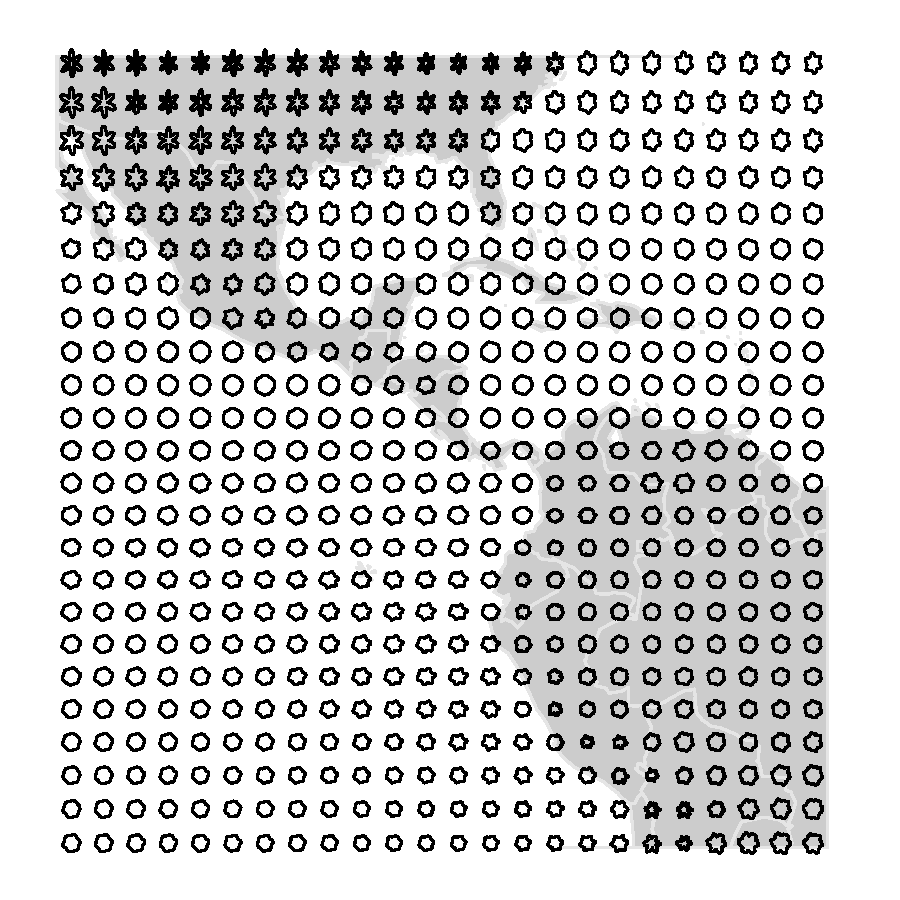
\includegraphics[width=3.5in]{nasa-glyph-all.pdf}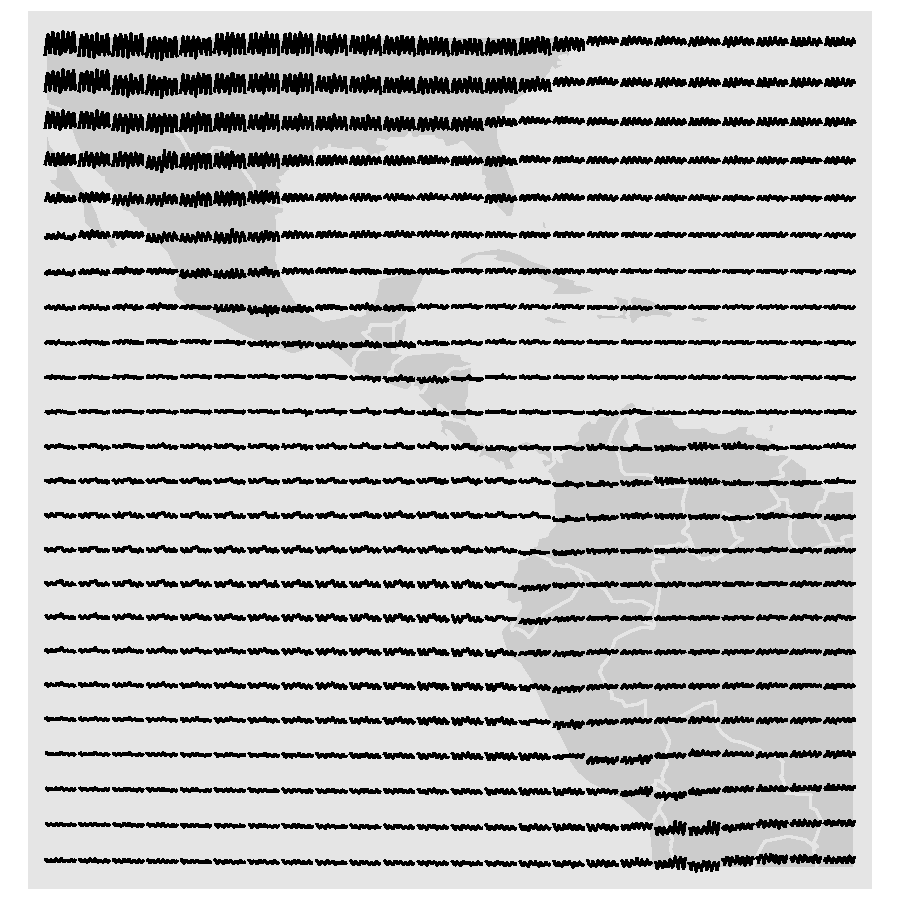
\includegraphics[width=3.5in]{nasa-glyph-ts-all.pdf}}
\caption{Glyph-map of raw data, using star glyphs (left), and time series as glyphs (right).}
\label{fig:glyph-map}
\end{figure*}

In this paper we describe the algorithm for creating glyphs of temporal data on maps, generally in R, and the various modifcations that can enable different features in the data to be detected. The next section (\ref{sec:construction}) describes how to construct glyph-maps. Section \ref{sec:reference} discusses the use of reference lines and boxes, and Section \ref{sec:scale} visits issues of scaling values for different information purposes. Generalizations to different types of icons are described in Section \ref{sec:scatter}. Glyph-maps work nicely with gridded data, but may be less effective with irregular spatial locations. Possible adjustments are discussed in Section \ref{sec:irregular}. Code and data is available in the online supplementary materials.
 
%\subsection{Glyph plots}

%Simple, but effective, technique that combines aspects of glyphs, facetted plots and map-charts. Particularly well suited for the type of temporal-spatial data, commonly seen in climate.

%Glyph-maps have attributes of both glyphs (stars, faces, profiles, ...), inviting exploration at the global level, and small-multiple time series, allowing local exploration of individual series. Allow to see both geographic context and individual locations simultaneously.

%Avoids one problem that plagues glyph displays: the ordering of the variables. Although some techniques exist to ameliorate this problem \citep{kleiner:1981,hurley:2010}, they are not necessary with time data because it is intrinsically ordered.

%These displays tend to be particularly effective when printed in large format, as the much higher resolution of print (600 dpi) compared to computer  screen (72-120 dpi) allows for much finer reading. These are high-density data displays in the best tradition of Tufte. Wall size maps are not usually practical during analysis, but are very engaging.

%Will first explore for regularly gridded data, a simple starting point and a common output of climate models, and then show a few simple extensions to deal with non-rectangular grids and irregular locations, as exemplified by raw climate data which is typically collect at irregular locations.

\section{Computation}~\label{sec:construction}

A big advantage of glyph-maps is that they can be generated with existing graphics software after performing a simple pre-processing step, making them easily accessible to a wide audience. The pre-processing step is simple, once you notice that the position of graphical elements is determined by a major and minor axis in each direction ($x$ and $y$). For maps, the major axes are latitude and longitude, and the minor axes are typically time and some measurement or model prediction. In addition, the minor axes are rescaled to have range $[0, 1]$. The final data values are a simple linear combination, as given by 

\begin{eqnarray*}\label{coords.eqn}
x_\text{ coordinate}&=& x_{\amaj} + w \cdot x_{\amin}\\
y_\text{ coordinate}&=& y_{\amaj} + h \cdot y_{\amin}
\end{eqnarray*}
where $w$ and $h$ are width and height respectively. The width and height will typically take into account the resolution of the major and minor axes, that is the minimum difference between consecutive locations.

Computing the coordinates for star glyphs is achieved by using polar coordinates,  $r=y_{\amin}$, and $\theta=x_{\amin}$, both scaled to be between 0 and 1. Then the glyph coordinates are given by 

\begin{eqnarray*}\label{coords.polar.eqn}
x_\text{ coordinate}&=& x_{\amaj} + \frac{w \cdot r}{2} \sin(2 \pi \theta)\\
y_\text{ coordinate}&=& y_{\amaj} + \frac{h \cdot r}{2} \cos(2 \pi \theta)
\end{eqnarray*}

Figure~\ref{fig:cycle} shows average monthly temperature as time (Cartesian coordinates) and star (polar coordinates) glyphs, for a subset of the spatial region. In this case, the star glyphs are not as effective as the linear glyphs: perhaps because of the absence of cyclical pattern.

\begin{figure}[htbp]
  \centering
  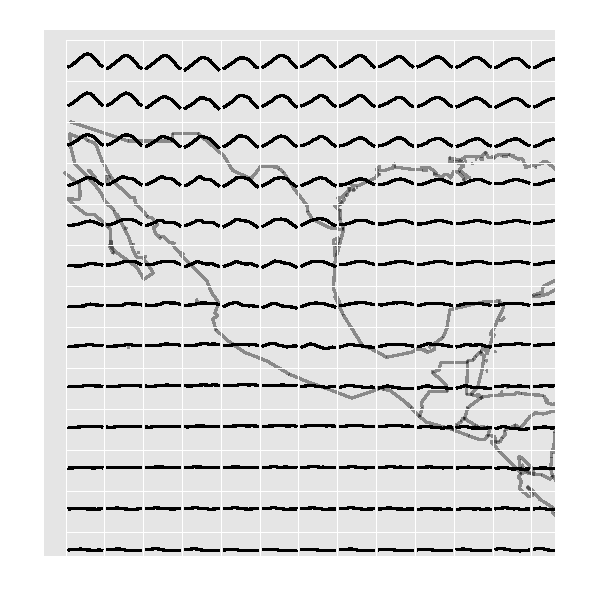
\includegraphics[width=3in]{month-cartesian}
  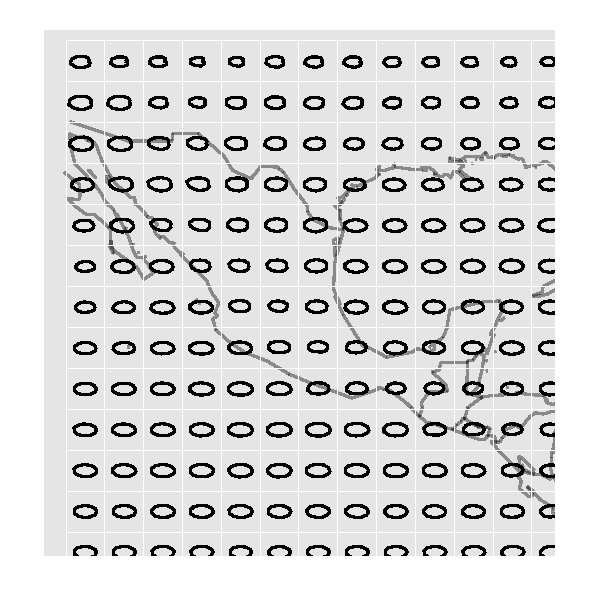
\includegraphics[width=3in]{month-polar}
    
  \caption{Monthly averages in (left) Cartesian coordinates and (right) polar coordinates.}
  
  \label{fig:cycle}
\end{figure}

Since the $x$ and $y$ locations are linear combinations of two variables, these types of displays can also be built interactively by software that supports tours \citep{cook:2006}, such as DataViewer \citep{buja:1986}, XGobi \citep{swayne:1991} or GGobi \citep{swayne:2003}.  This technique is used to good effect in \citet{buja:1996a}.

% Show the glyph-map for de-seasonalized data, and describe what we
% see differently from the facetted map

The graphics in this paper were created in R \citep{R} using {\tt ggplot2} \citep{me:ggplot2} and {\tt plyr} \citep{me:plyr}. 

\section{Reference lines}~\label{sec:reference}

Graphical displays benefit from a \emph{visual reference grid} \citep{cleveland:1993a} to compare values mapped to position along a line. The same is true for glyph-maps, but it is not feasible to make a full set of axies for each icon. A complete axis would dominate the picture, and draw the eye away from the pattern of the data. The types of comparisons that are needed across icons are:

\begin{itemize} \itemsep 0in
\item Slope, or trend
\item Intercept, or average value
\item Variance, or size
\end{itemize}

Space-time-glyphs usually require a  to make it easier to compare locations. This is important for accurate perception of important line properties like slope and minima. This need is evident in Figure~\ref{fig:glyph-map}. There is a hint that the average value is not the same from right time series to the next in the map (right), or if the center of the icons is the same in the polar time series (left). We have no frame of reference on which to judge this. The regular grid provides a very rudimentary frame of reference, but it is not sufficient. 

Figure~\ref{fig:ref-basic} shows two reference grid variants: a line drawn at the overall mid-range, and a box drawn around each grid cell. We prefer using white for these references because it is minimally perceptible: you can see the grid easily when looking for it, but it does not otherwise distract from the perception of the graphic \citep{carr:1994}. When we add a reference to each location, as in Figure~\ref{fig:ref-basic}, we see not only a difference in shape between Northern and Southern hemispheres, but also average value. Without reference lines, it is difficult to see that average seasonal coefficients are much higher in the North than in the South.

% Think we might need to show the original figures of data with reference lines

\begin{figure}[htbp]
  \centering
  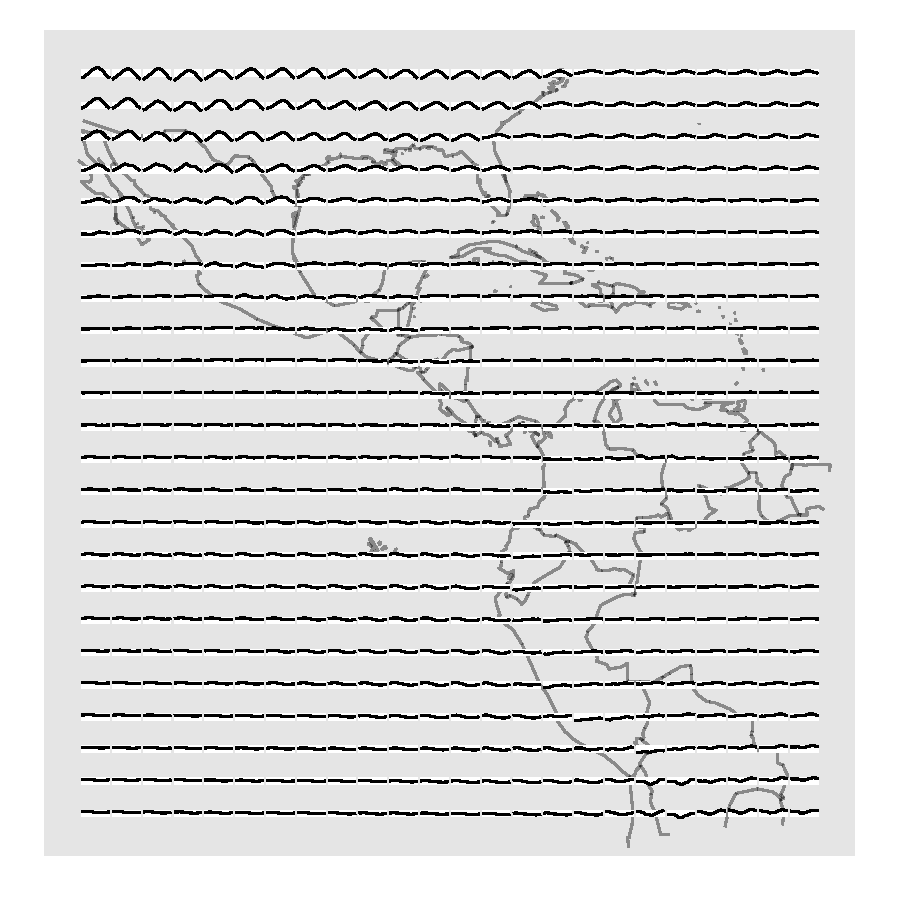
\includegraphics[width=0.5\linewidth]{ref-line}%
  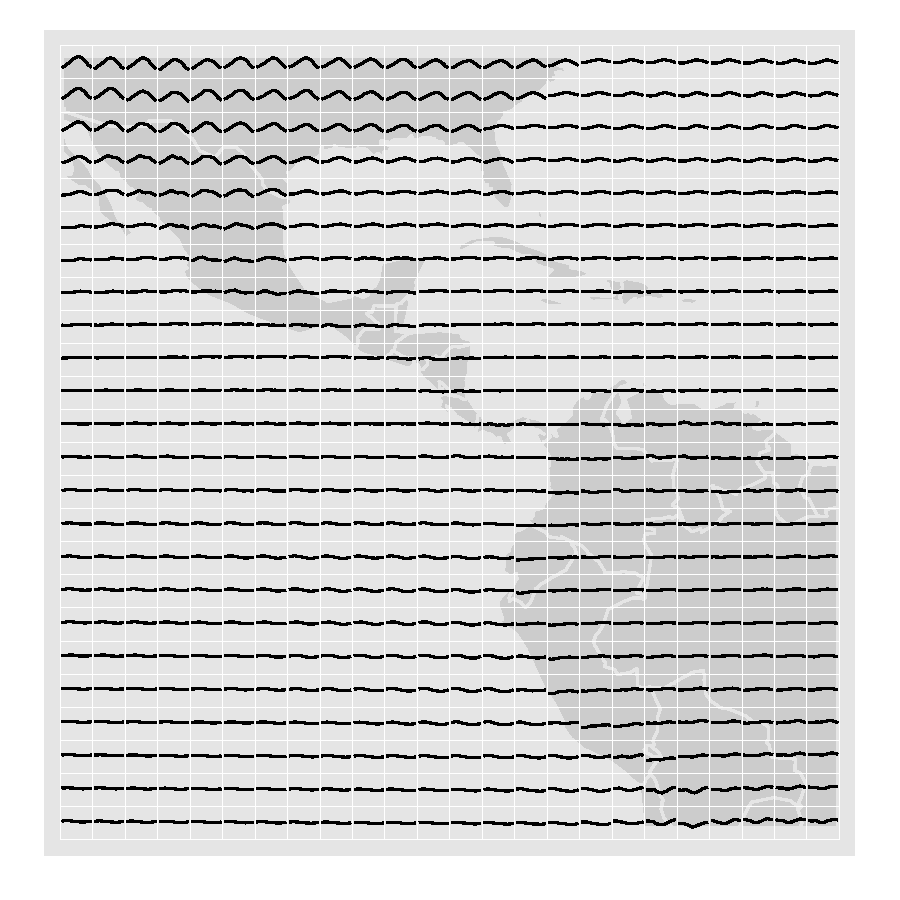
\includegraphics[width=0.5\linewidth]{ref-box}

  \caption{Glyph-maps of seasonal temperature patterns. Adding reference lines, (left) mid-range lines and (right) grid-cell boxes, makes it easier to see differences in glyph position, not just shape.}
  \label{fig:ref-basic}
\end{figure}

It's also often useful to display other types of reference information. You are only limited by your imagination (and the capabilities of your graphics software), but two simple ideas are to (1) vary the colour or transparency of glyphs or references, or (2) use an additional layer to highlight special points. Figure~\ref{fig:ref-adv} illustrates these ideas to display the month with the highest temperature at each locations. Careful colour choice is necessary so that this information is perceptible, but not distracting.

\begin{figure}[htbp]
  \centering
  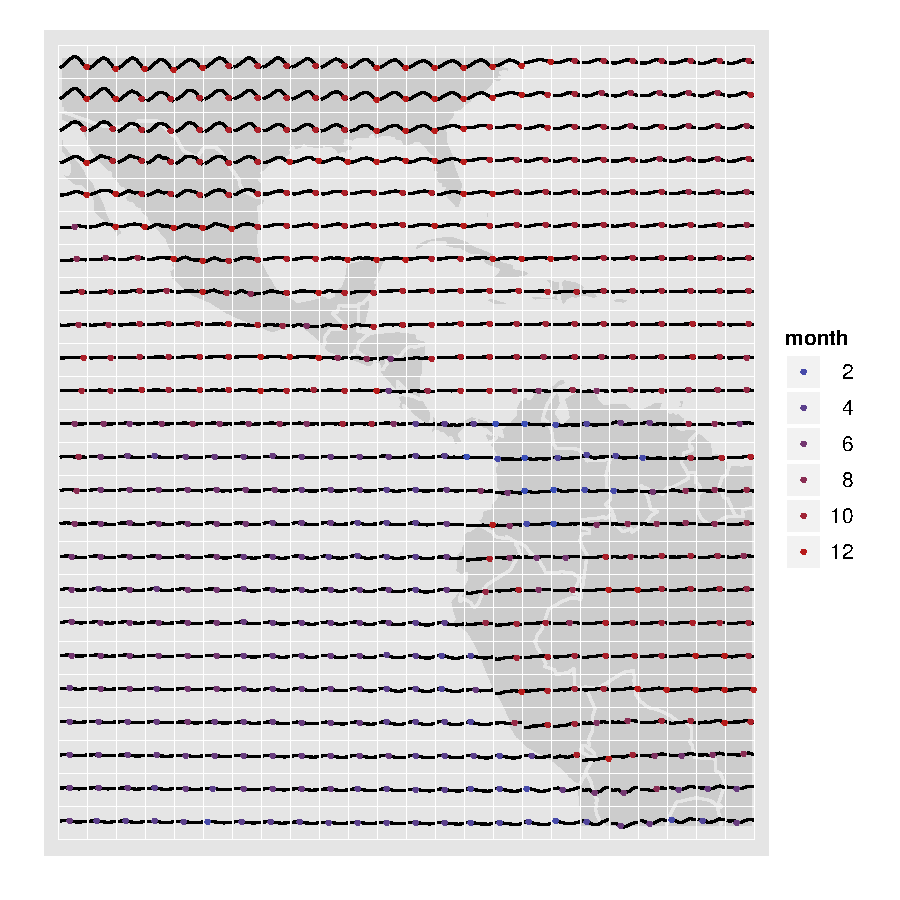
\includegraphics[width=0.5\linewidth]{ref-max-1}%
  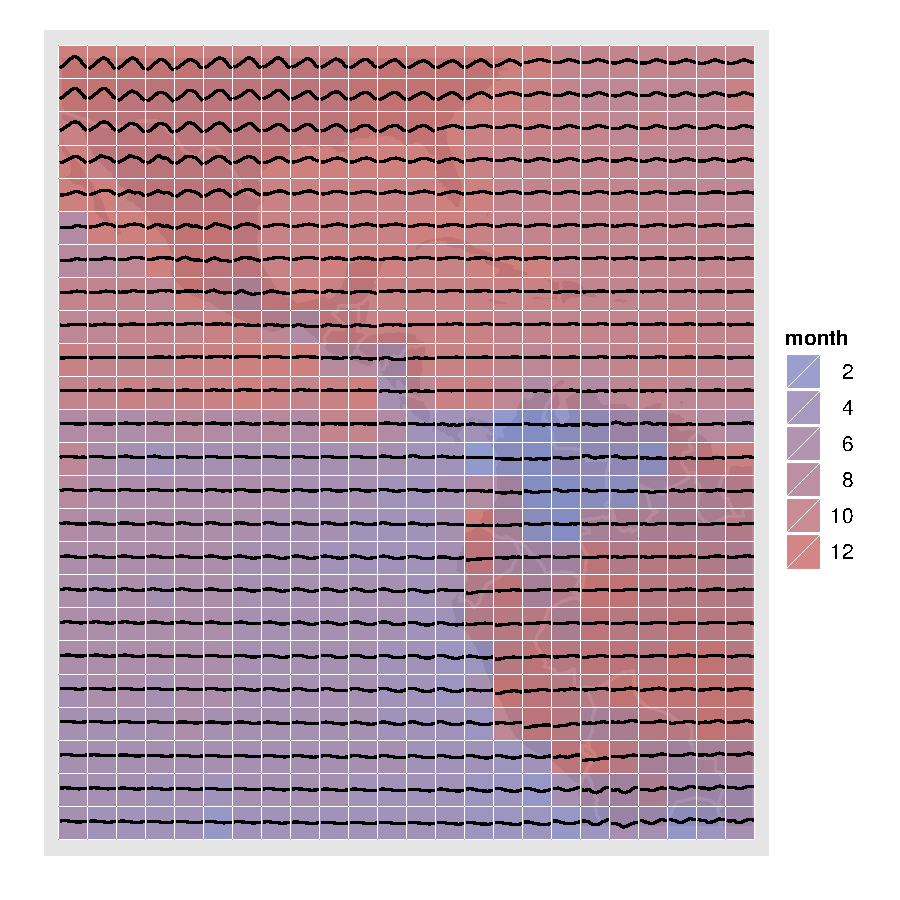
\includegraphics[width=0.5\linewidth]{ref-max-2}
  \caption{Glyph-maps of seasonal temperature patterns also showing the month with the highest temperature using (left) an additional layer of points and (right) changing the background colour of the reference grid.}
  \label{fig:ref-adv}
\end{figure}

A particularly useful summary when to add when displaying model predictions, is some measure of model fit. This makes it easier to avoid over-interpreting predictions from poorly-fitting models.

\section{Perception of structure}~\label{sec:scale}

Compare the facetted map Fig 1 with the glyph-map of de-seasonalized data

\section{Partitioning patterns into shape and size}~\label{sec:scale}

*** This section might benefit from some equations also.

Another impact of varying averages is that it tends to diminish the perceptibility of shape: if some series have uniformly high values and some have uniformly low, then it is difficult to see if the shape is the same independent of the average. Partitioning is a extremely useful technique: product plots, ANOVA, ...  For glyph plots, it's often useful to partition the glyphs into shape and scale components, decomposing the values into a product of maximum and scaled values.  In this section we explore how decomposing each series into scale and shape components can be useful.

This is revealing for smooth models of surface temperature, shown in Figure~\ref{fig:scaling}. Each location is modelled using a generalised additive model \citep{wood:2006} with a seasonal term and a long-term smooth term. The three plots in the figure show the long-term smooth term. Because some locations are uniformly warmer than others, the impact of changes across time are diminished. In the centre plot, each location is scaled by dividing out the maximum, and on the right, each location is scaled to range $[0, 1]$. These emphasise individual changes but lose the ability to make global comparisons, and need caution when interpreting - a small absolute change gets blown up into a large relative change.

\begin{figure}[htbp]
  \centering
  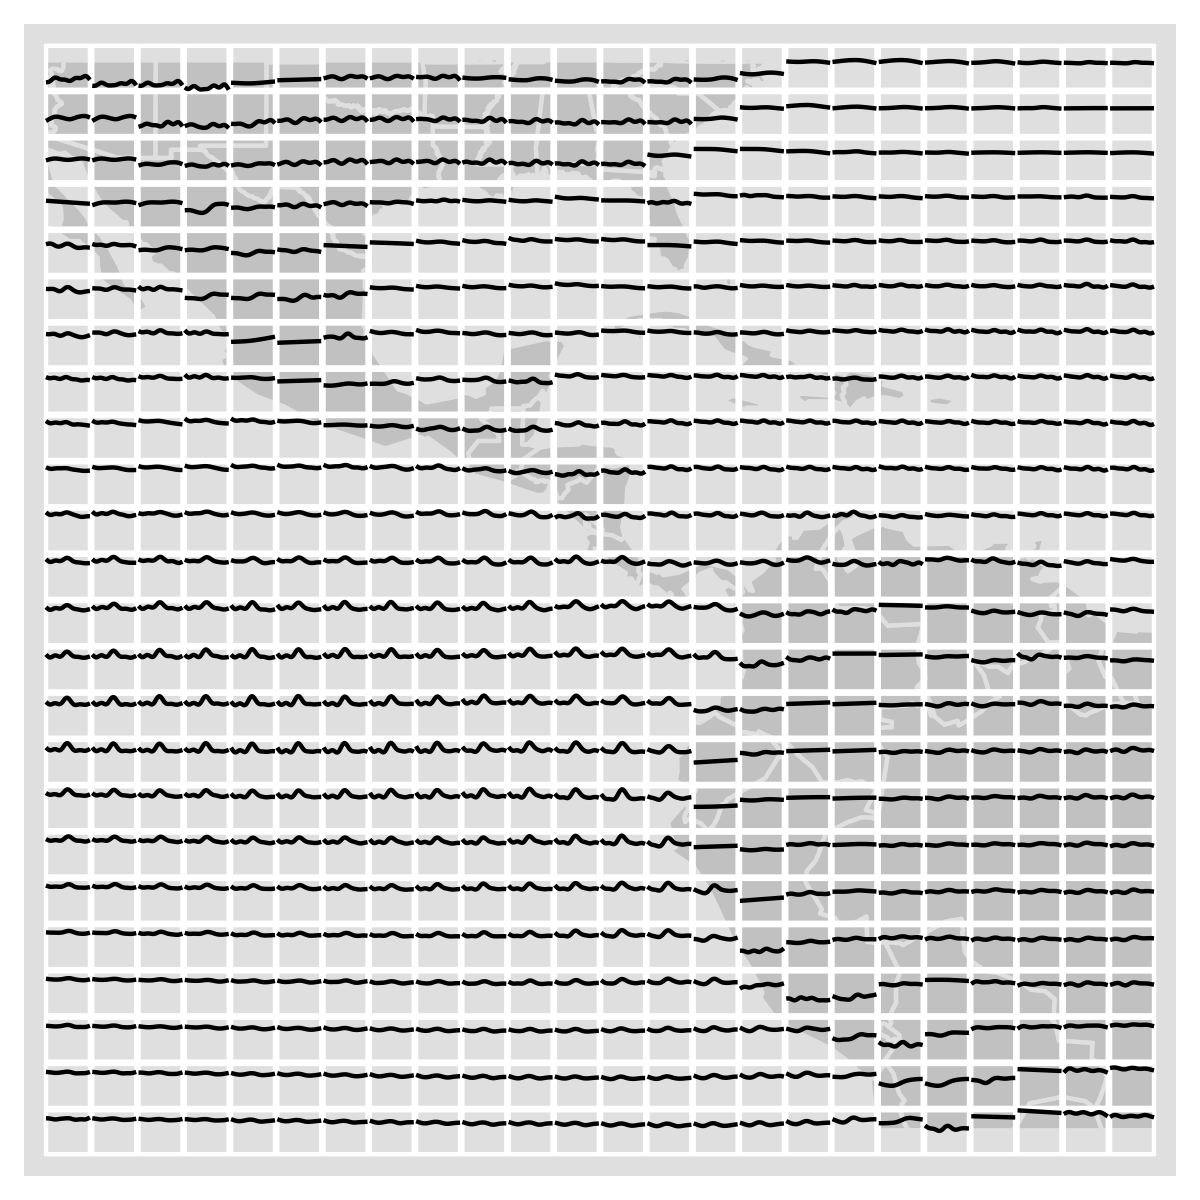
\includegraphics[width=0.33\linewidth]{month-rescale-none}%
  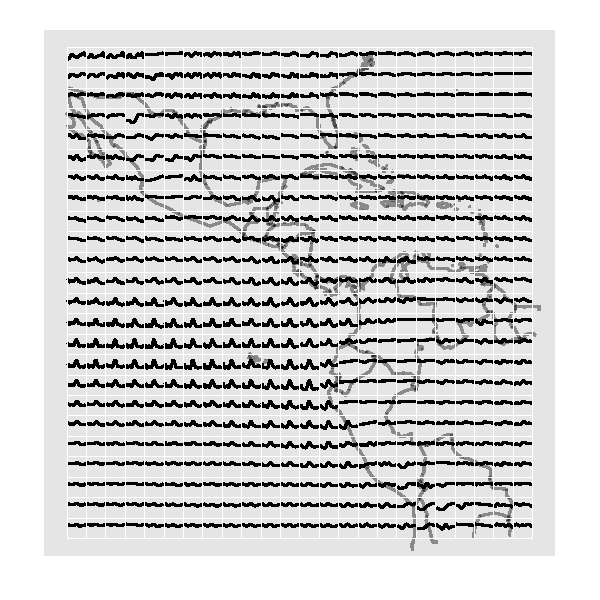
\includegraphics[width=0.33\linewidth]{month-rescale-max}%
  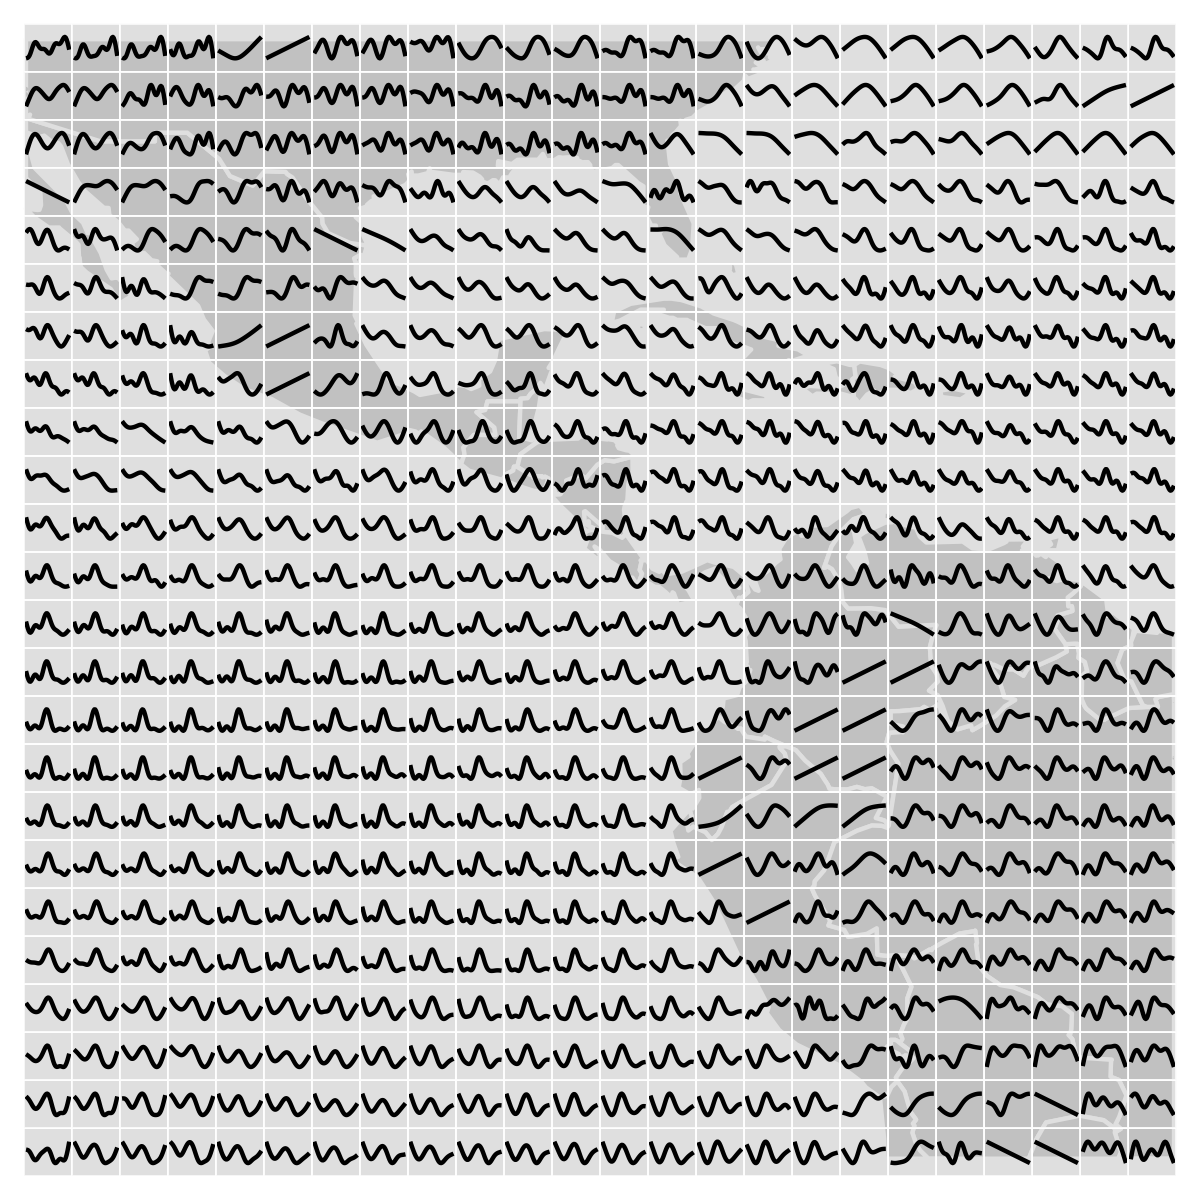
\includegraphics[width=0.33\linewidth]{month-rescale01}
  \caption{Smoothed de-seasonalized daily temperature glyph-map. (Left) unscaled, (center) scaled to have maximum 1, (right) scaled to have maximum 1 and minimum 0.}
  \label{fig:scaling}
\end{figure}

A possible compromise is to use line colour to display the standardising variable, as shown in Figure~\ref{fig:scaling-col}.  This makes it possible to see the individual patterns while still retaining some ability to see which shapes represent small absolute changes.

\begin{figure}[htbp]
  \centering
  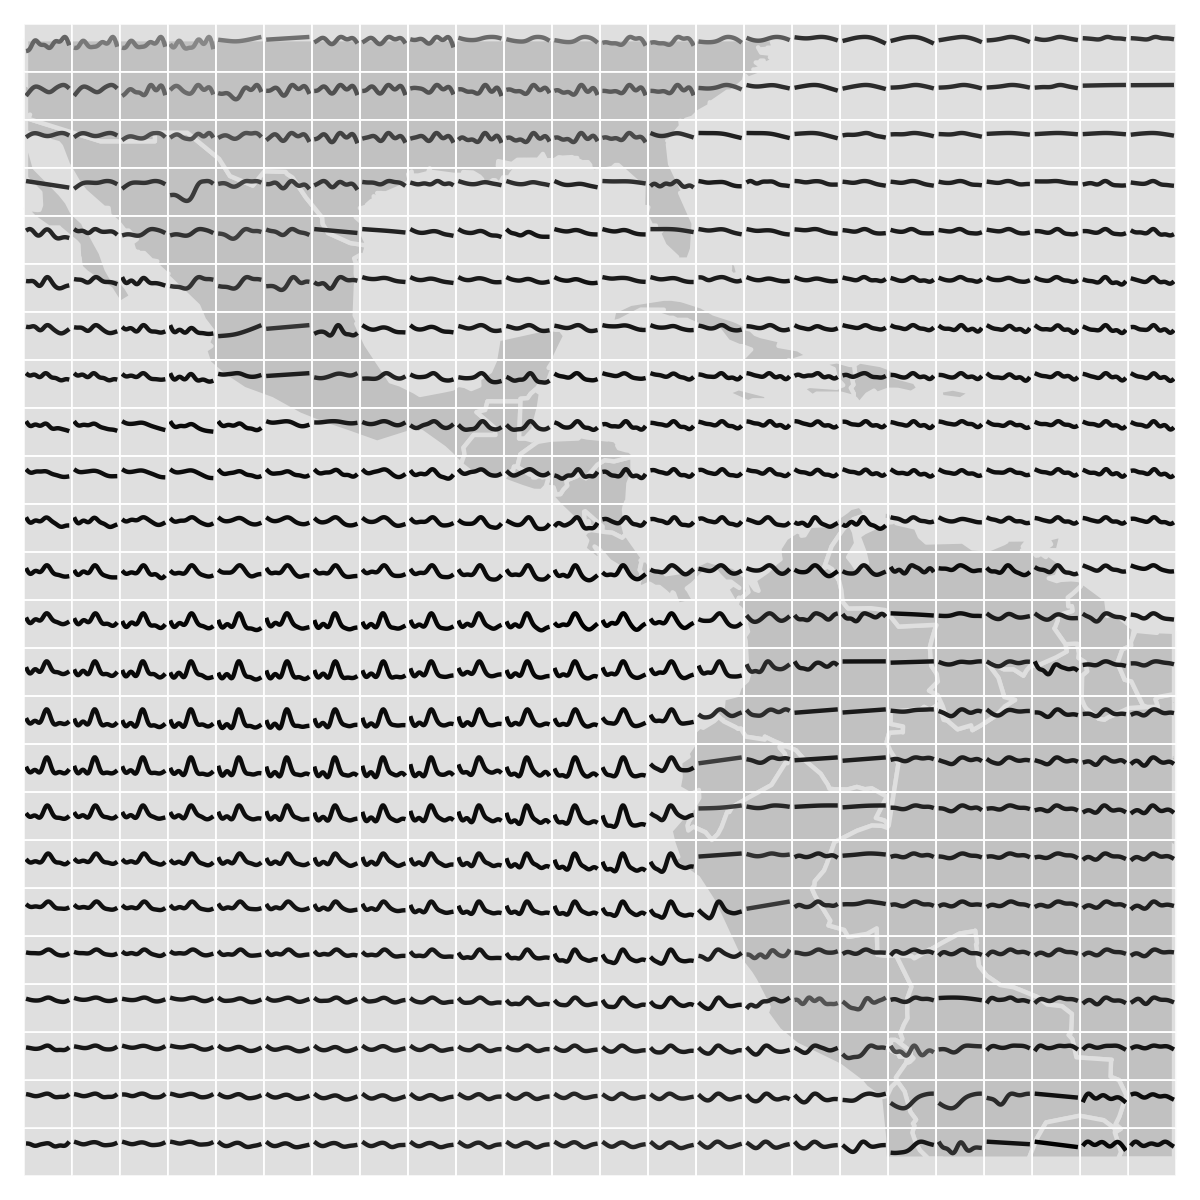
\includegraphics[width=0.33\linewidth]{month-rescale01-col}
  \caption{Adding colour to scaled plots. Here each location has been scaled to range $[0, 1]$ and colour mapped to the range of the original predictions.}
  \label{fig:scaling-col}
\end{figure}

Of course other types of scaling are possible. Another classical scaling method is to standardize mean and standard deviation to 0 and 1 (or robust variants).

Equivalent to using individual scales in facetted graphics. 

\section{What to plot: raw data, trend lines, residuals,  seasonal}

\section{Generalization: scatterplots}~\label{sec:scatter}

So far we have limited ourselves to always mapping some aspect of time on the x-axis. But glyph-maps are not limited to only this type of data and can  be easily generalized to create many other types of display. Figure~\ref{fig:cloud} shows a generalisation to scatterplots: by mapping another variable to the x-axis, in this case low-cloud level on x and high-cloud level on y, we can explore how a bivariate relationship varies spatially. It is again useful to use a model to extract the essence of the relationship, summarizing the data with models is very useful: the second plot displays a loess curve fit to the data instead of the individual points.  

\begin{figure}[htbp]
  \centering
  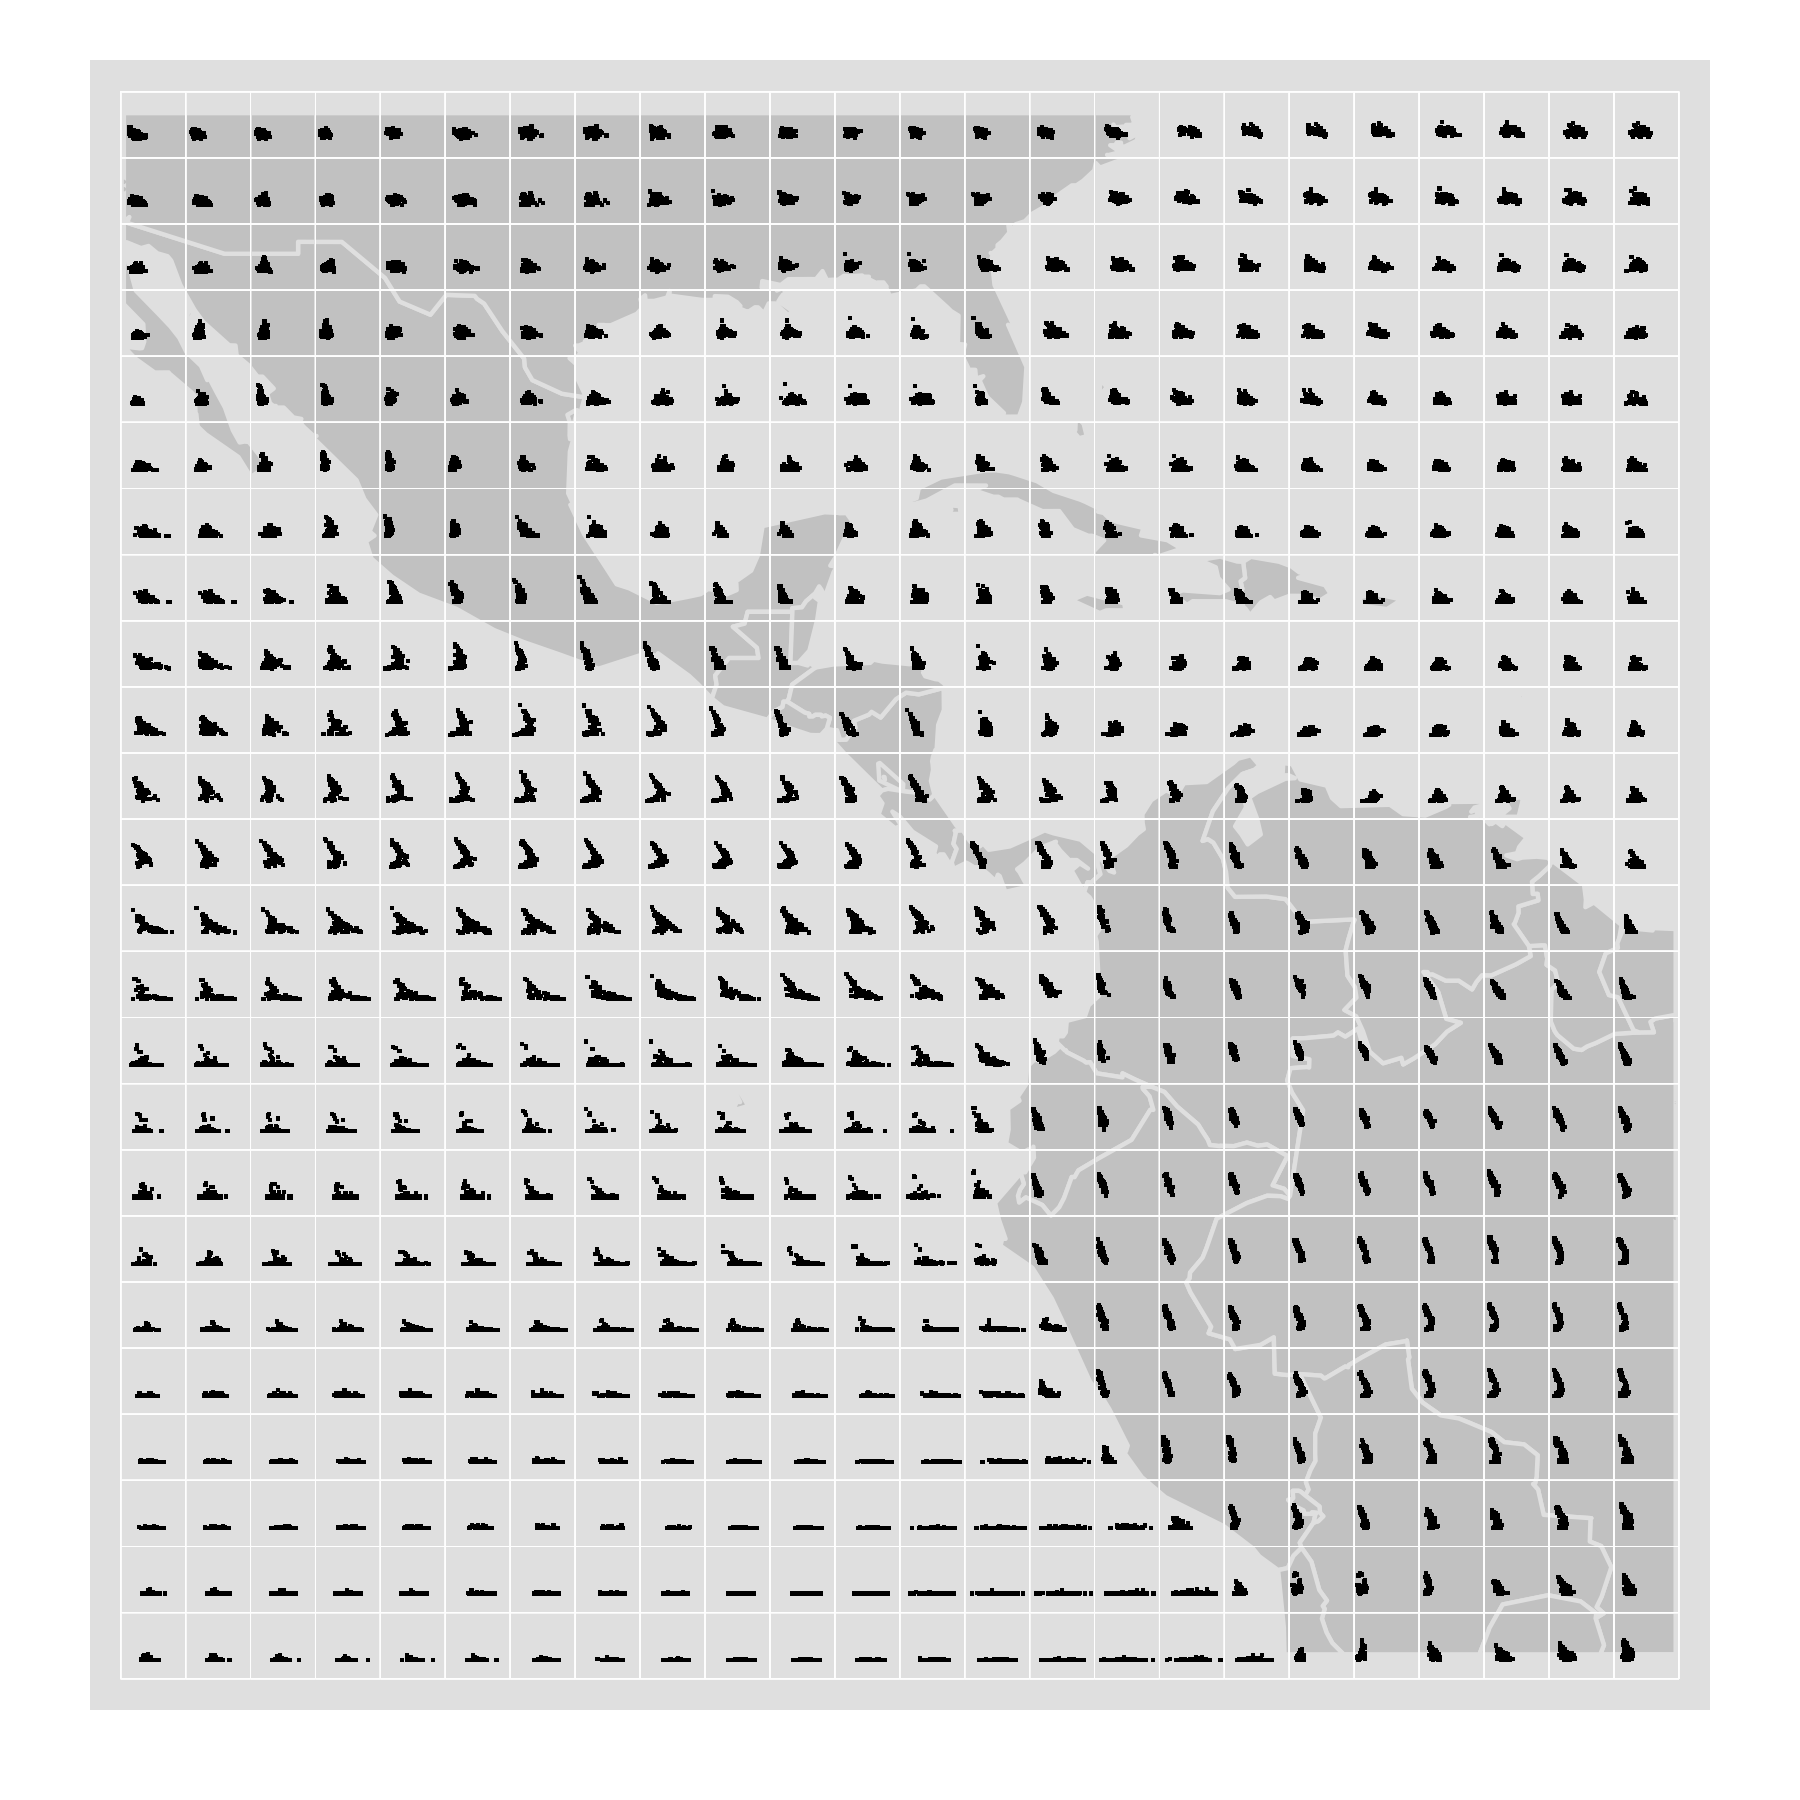
\includegraphics[width=0.5\linewidth]{clouds}%
  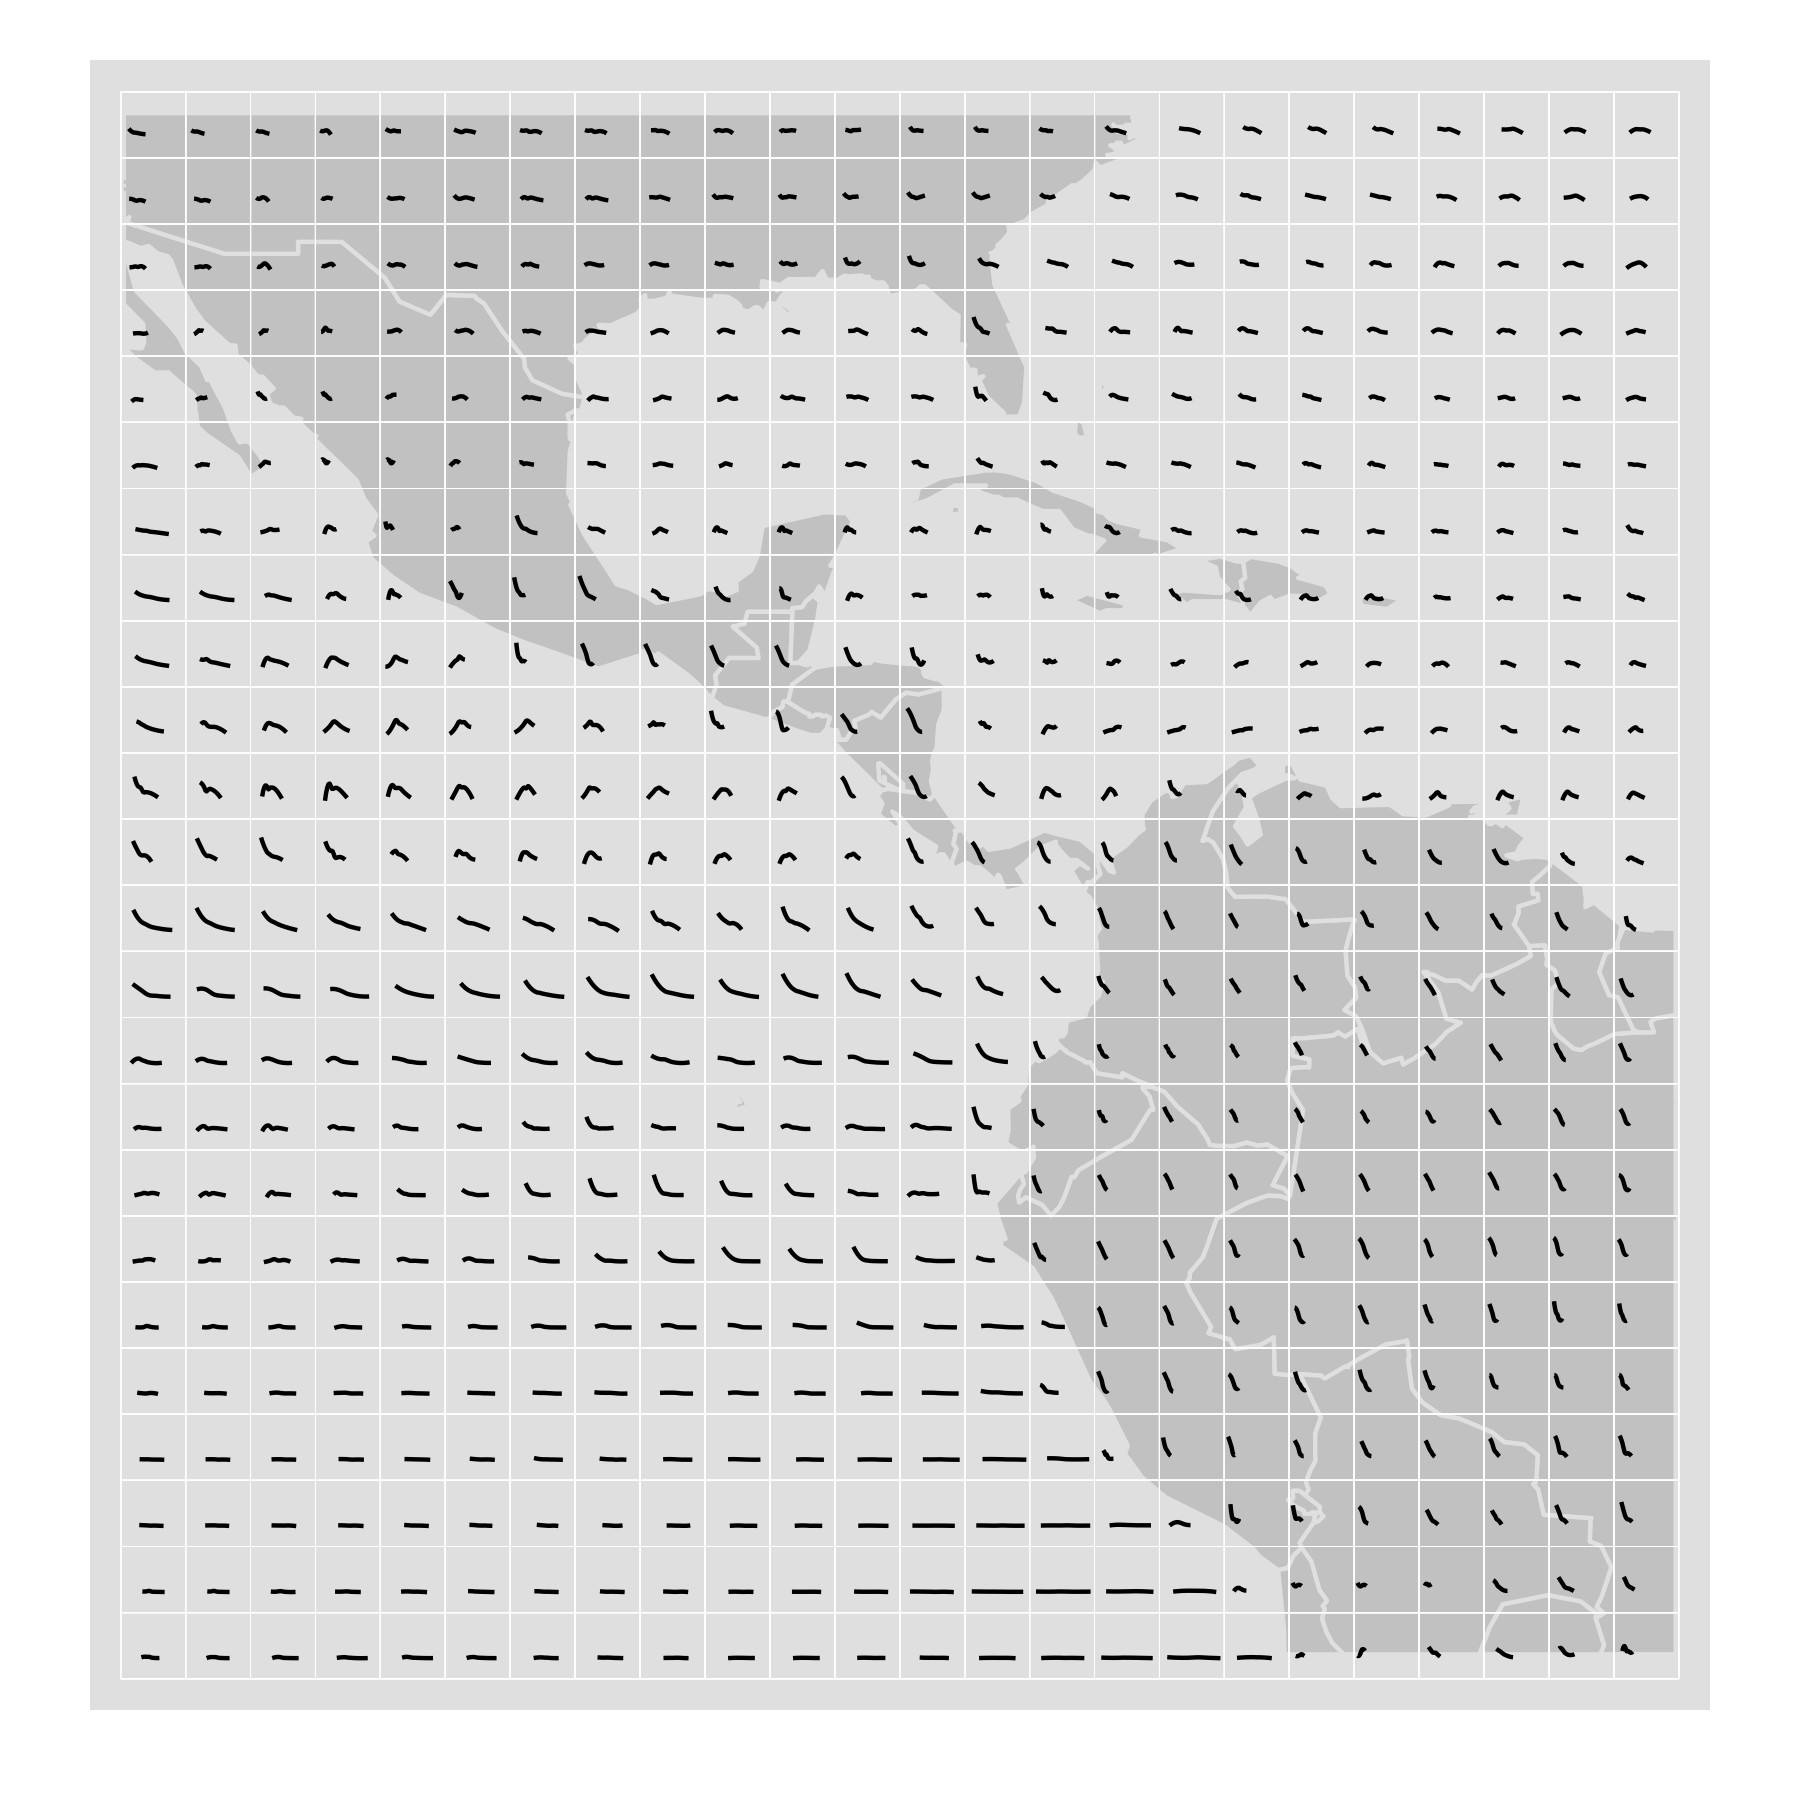
\includegraphics[width=0.5\linewidth]{clouds-smooth}

  \caption{Glyph-map showing (left) scatterplot of high-cloud vs. low-cloud and (right) smoothed (loess) curve fit to each location. The relationship between these two variables varies considerably over the spatial domain (particularly between land and ocean), but neighbouring locations tend to similar. }
  \label{fig:cloud}
\end{figure}


\section{Regular vs irregular locations}~\label{sec:irregular}

\subsection{Non-rectangular grids}

Rectangular, but not in this projection.  Other types of regular grids.

\subsection{Irregular locations}

\section{Long time series}

\section{Conclusions}

\bibliography{references}

\end{document}